%% Default Latex document template
%%
%%  blake@rcs.ee.washington.edu

\documentclass[letterpaper]{article}

% Uncomment for bibliog.
%\bibliographystyle{unsrt}

\usepackage{graphicx}
% \usepackage{lineno}
%\usepackage{fancyhdr}

%%%%%%%%%%%%%%%%%%%%%%%%%%%%%%%%%%%%%%%%5
%
%  Set Up Margins
\input{templates/pagedim.tex}

%
%        Font selection
%
%\renewcommand{\rmdefault}{ptm}             % Times
%\renewcommand{\rmdefault}{phv}             % Helvetica
%\renewcommand{\rmdefault}{pcr}             % Courier
%\renewcommand{\rmdefault}{pbk}             % Bookman
%\renewcommand{\rmdefault}{pag}             % Avant Garde
%\renewcommand{\rmdefault}{ppl}             % Palatino
%\renewcommand{\rmdefault}{pch}             % Charter


%%%%%%%%%%%%%%%%%%%%%%%%%%%%%%%%%%%%%%%%%%%%%%%%%
%
%         Page format Mods HERE
%
%Mod's to page size for this document
\addtolength\textwidth{0cm}
\addtolength\oddsidemargin{0cm}
\addtolength\headsep{0cm}
\addtolength\textheight{0cm}
%\linespread{0.894}   % 0.894 = 6 lines per inch, 1 = "single",  1.6 = "double"

%\lhead{LEFT HEADER}
%\chead{CENTER HEADER}
%\rhead{RIGHT HEADER}
%\lfoot{Hannaford, U. of Washington}
%\rfoot{\today}
%\cfoot{\thepage}

% Make table rows deeper
%\renewcommand\arraystretch{2.0}% Vertical Row size, 1.0 is for standard spacing)
\usepackage{tikz}
\usetikzlibrary{calc,patterns,decorations.pathmorphing,decorations.markings,calc}

\usetikzlibrary{circuits}
\usetikzlibrary{circuits.ee.IEC}

\begin{document}
% \setpagewiselinenumbers        %  Line numbers for edits to drafts.
% \modulolinenumbers[1]          %  number every N lines

% \linenumbers                   %  start numbering lines here
% %
%  \begin{tikzpicture}[every node/.style={draw,outer sep=0pt,thick}]
% %
% % % Spring
%  \tikzstyle{spring}=[thick,decorate,decoration={zigzag,pre length=0.3cm,post length=0.3cm,segment length=6}]
% %
% % % Damper
%  \tikzstyle{damper}=[thick,decoration={markings,
%    mark connection node=dmp,
%    mark=at position 0.5 with
%    {
%      \node (dmp) [thick,inner sep=0pt,transform shape,rotate=-90,minimum width=15pt,minimum height=3pt,draw=none] {};
%      \draw [thick] ($(dmp.north east)+(2pt,0)$) -- (dmp.south east) -- (dmp.south west) -- ($(dmp.north west)+(2pt,0)$);
%      \draw [thick] ($(dmp.north)+(0,-5pt)$) -- ($(dmp.north)+(0,5pt)$);
%    }
%  }, decorate]
% %
% % Ground
%  \tikzstyle{ground}=[fill,pattern=north east lines,draw=none,minimum width=0.75cm,minimum height=0.3cm]
% %
% %
%  \node (M) [minimum width=3.5cm,minimum height=2cm] {$m_1$};
% %
% % %  left most spring ground
%  \node (ground1) at (M.south) [ground,yshift=-1.5cm,xshift=-1.25cm,anchor=north] {};
%  \draw (ground1.north west) -- (ground1.north east);
%  \draw [spring] (ground1.north) -- ($(M.south east)!(ground1.north)!(M.south west)$);
% %
%  % damper ground
%  \node (ground2) at (M.south) [ground,yshift=-1.5cm,anchor=north] {};
%  \draw (ground2.north west) -- (ground2.north east);
%  \draw [damper] (ground2.north) -- ($(M.south east)!(ground2.north)!(M.south west)$);
% %
%  % right spring ground
%  \node (ground3) at (M.south) [ground,yshift=-1.5cm,xshift=1.25cm,anchor=north] {};
%  \draw (ground3.north west) -- (ground3.north east);
%  \draw [spring] (ground3.north) -- ($(M.south east)!(ground3.north)!(M.south west)$);
% %
% % % up arrow vector
%  \draw [-latex,ultra thick] (M.north) ++(0,0.2cm) -- +(0,1cm);
% %
% %
% % %%%%%%%%%%%%%%%%%%%%%%%%%%%%%%%%%%%%%%%%%
%  \begin{scope}[xshift=7cm]
%  \node (M) [minimum width=1cm, minimum height=2.5cm] {$m$};
%
%  \node (ground) [ground,anchor=north,yshift=-0.25cm,minimum width=1.5cm] at (M.south) {};
%  \draw (ground.north east) -- (ground.north west);
% %
% % % little wheels
%  \draw [thick] (M.south west) ++ (0.2cm,-0.125cm) circle (0.125cm)  (M.south east) ++ (-0.2cm,-0.125cm) circle (0.125cm);
% %
%  \node (wall) [ground, rotate=-90, minimum width=3cm,yshift=-3cm] {};
%  \draw (wall.north east) -- (wall.north west);
% %
%  \draw [spring] (wall.170) -- ($(M.north west)!(wall.170)!(M.south west)$);
%  \draw [damper] (wall.10) -- ($(M.north west)!(wall.10)!(M.south west)$);
% %
%  \draw [-latex,ultra thick] (M.east) ++ (0.2cm,0) -- +(1cm,0);
%  \end{scope}
%  \end{tikzpicture}
% %
%



%%%%%%%%%%%%%%%%%%%%%%%%%%%%%%%%%%%%%%%%%%%%%%%%%%%%%%%%%%%%%%%%%%%%%%%%%%%%%%%%%%%%%%%%

%           Vibrotactile Actuator Diagram

%%%%%%%%%%%%%%%%%%%%%%%%%%%%%%%%%%%%%%%%%%%%%%%%%%%%%%%%%%%%%%%%%%%%%%%%%%%%%%%%%%%%%%%%

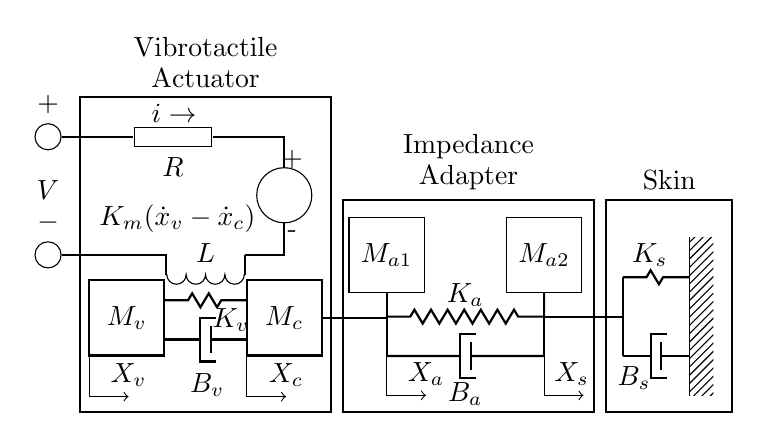
\begin{tikzpicture}[circuit ee IEC, every node/.style={draw, thick,outer sep=0pt,thick}]

% debugging grid
% \draw[step=5mm,gray,very thin] (-25mm,-25mm) grid (100mm,50mm);
% \draw[thick,gray] (0,-25mm) -- (0,50mm);
% \draw[thick,gray] (-25mm,0) -- (100mm,0);



% Spring
\tikzstyle{spring}=[thick,decorate,decoration={zigzag,pre length=0.3cm,post length=0.3cm,segment length=6}]

% Damper
\tikzstyle{damper}=[thick,decoration={markings,
  mark connection node=dmp,
  mark=at position 0.5 with
  {
    \node (dmp) [thick,inner sep=0pt,transform shape,rotate=-90,minimum width=15pt,minimum height=3pt,draw=none] {};
    \draw [thick] ($(dmp.north east)+(2pt,0)$) -- (dmp.south east) -- (dmp.south west) -- ($(dmp.north west)+(2pt,0)$);
    \draw [thick] ($(dmp.north)+(0,-5pt)$) -- ($(dmp.north)+(0,5pt)$);
  }
}, decorate]

% Ground
\tikzstyle{ground}=[fill,pattern=north east lines,draw=none,minimum width=0.75cm,minimum height=0.3cm]


%%%%%%%%%%%%%%%%%%%%%%%%%%%%%%%%%%%%%%%%%%%%%%%%%%%%%%%%%%%%%%%55
%
%       System Layout
%
\node (actuator) [minimum width=31.8mm, minimum height=40mm, anchor=south] {};
\node (adapter) [minimum width=31.8mm, minimum height=27mm, xshift=33.4mm, yshift=0, anchor=south] {};
\node (skin) [minimum width=16mm,   minimum height=27mm, xshift=58.9mm, yshift=0, anchor=south] {};

%%%%%%%%%%%%%%%%%%%%%%%%%%%%%%%%%%%%%%%%%%%%%%%%%%%%%%%%%%%%%%%%%%%%
%
%        Vibrotactile Actuator
%
\node (Mv) [minimum width=.955cm,minimum height=.955cm, xshift=-10mm, yshift=12mm] {$M_v$};
\node (Mc) [minimum width=.955cm,minimum height=.955cm, xshift= 10mm, yshift=12mm] {$M_c$};

\tikzstyle{every node}=[];


\node[above, yshift=4mm] at (actuator.north)  {Vibrotactile};
\node[above]             at (actuator.north)  {Actuator};
\node[above,yshift=4mm] at (adapter.north)   {Impedance};
\node[above] at (adapter.north)   {Adapter};
\node[above] at (skin.north)      {Skin};

\draw [->] (Mv.west) -- ++(0,-10mm) -- ++(5mm,0) node[above] {$X_v$};
\draw [->] (Mc.west) -- ++(0,-10mm) -- ++(5mm,0) node[above] {$X_c$};


%%%%%%%%%%%%%%%%%%%%%%%%%%%%%%%%%%%%%%%%%%%%%%%%%%%%%%%%%%%%%%
%
%        Electrical Loop

\node (EMF)  [circle, draw,minimum width=7mm, above, yshift=12mm] at (Mc){};
\node  ()    [xshift=-10mm,yshift=-3mm] at (EMF.west) {$K_m(\dot{x}_v-\dot{x}_c)$};
\node  ()    [xshift=1mm, yshift=1mm] at (EMF.north) {+};
\node  ()    [xshift=1mm, yshift=-1mm] at (EMF.south) {-};
\node (V1)   [circle,draw,minimum width=0.1cm ] at (-20mm,20mm) {};
\node (V2)   [circle,draw,minimum width=0.1cm ] at (-20mm,35mm) {};
\node () [above] at (V1.north) {$-$};
\node () [above,yshift=4mm] at (V1.north) {$V$};
\node () [above] at (V2.north) {$+$};
\node () [xshift=-4mm]      at (0mm,38mm)  {$i\to$};
%%%%%%%55
% inductor
\coordinate (L1a)   at  (-5mm,17.5mm) {};
\coordinate (L1a2)  at  (-5mm,  20mm) {};
\coordinate (L1b)   at  ( 5mm,17.5mm) {};
\coordinate (L1b2)  at  ( 5mm,  20mm) {};

% wiring, R, L
\draw[thick]  (V1) -- (L1a2) -- (L1a); %
\draw[thick]  (V2) to[resistor={info'=$R$}] (10mm,35mm) -- (EMF.north);
\draw[thick]  (EMF.south) -- (10mm,20mm) -- (L1b2);
\draw[thick]  (L1b2) -- (L1b); % ;
\draw[thick]  (L1b) to[inductor={info'=$L$}, rotate=180] (L1a);




%%%%%%%%%%%%%%%%%%%5
%  actuator spring-damper
\draw [spring] (Mv.25)  -- ($(Mc.north west)!(Mv. 25)!(Mc.south west)$);
\node () at ($(Mc.north west)+(-2mm,-5mm)$) {$K_v$};
\draw [damper] (Mv.-30) -- ($(Mc.north west)!(Mv.-30)!(Mc.south west)$) node[below,xshift=-5mm,yshift=-3mm]  {$B_v$};

\begin{scope}[xshift=33mm]

\node (Ma1) [draw, minimum width=.955cm, minimum height=.955cm, xshift=-10mm, yshift=20mm] {$M_{a1}$};
\node (Ma2) [draw, minimum width=.955cm, minimum height=.955cm, xshift= 10mm, yshift=20mm] {$M_{a2}$};

\end{scope}

% \node[circle, fill=black, minimum size=1mm] (Xa) at (10mm,10mm) {};
% \draw[black] ($(Mc.north east)$) circle [radius=1mm-0.5\pgflinewidth,fill=black];

\draw [thick] let \p1=(Mc), \p2=(Ma1.south) in (Mc.east) -- (\x2,\y1);
\draw [thick] let \p1=(Mc), \p2=(Ma1.south) in (\x2,\y1) -- (\x2,\y2);


% % Nodes for imp adapter
% \fill ($(Ma1.south)-(0,3mm)$)   circle (2pt) node[name=Xa] {};
% \fill ($(Xa)+(20mm,0)$)         circle (2pt) node[name=Xs] {};
\coordinate (Xa)  at ($(Ma1.south)-(0,3mm)$)    {};
\coordinate (Xs)  at ($(Xa)+(20mm,0)$)          {};
\coordinate (Xa1) at ($(Ma1.south)-(0,8mm)$)    {};
\coordinate (Xs1) at ($(Xa)+(20mm,-5mm)$)       {};

\draw [->] (Xa1.south) -- ++(0,-5mm) -- ++(5mm,0) node[above] {$X_a$};
\draw [->] (Xs1.south) -- ++(0,-5mm) -- ++(5mm,0) node[above,xshift=-1.5mm] {$X_s$};

% \fill   circle (2pt) node[name=Xa1] {};
% \fill         circle (2pt) node[name=Xs1] {};



\node  (Xs2) at ($(Xs)+(10mm,0)$) {};
\node  (Xs3) at ($(Xs)+(10mm,5mm)$) {};
\node  (Xs4) at ($(Xs)+(10mm,-5mm)$) {};

\draw[thick] (Xs) -- ($(Xs)+(10mm,0)$) --  ($(Xs)+(10mm,5mm)$) --($(Xs)+(10mm,-5mm)$);


% Imp adapter K,B
 \draw[thick] (Xs) -- (Ma2.south);
 \draw[thick] (Xs) -- (Xs2);
 \draw[thick] (Xa) -- (Xa1);
 \draw[thick] (Xs) -- (Xs1);
\draw [spring] (Xa)   -- (Xs)  node[above,xshift=-10mm]  {$K_a$};
\draw [damper] (Xa1)  -- (Xs1) node[below,xshift=-10mm,yshift=-2mm]  {$B_a$};
% \node () at ($(Mc.north west)+(-2mm,-4mm)$) {$K_v$};
% skin K,B
\node (bone) [ground, rotate=90, minimum width=2.0cm] at ($(Xs2)+(10mm,0)$) {};
\draw (bone.north east) -- (bone.north west);


\draw[thick]   (Xs3) -- (Xs4);
\draw [spring] ($(Xs)+(10mm, 5mm)$)    -- (bone.north|-Xs3) node[above,xshift=-5mm] {$K_s$};
\draw [damper] ($(Xs)+(10mm,-5mm)$)    -- (bone.north|-Xs4) node[below,xshift=-7mm] {$B_s$};
% \draw [damper] (Xa1)  -- (Xs1);





% \draw [thick] (Mc.east)  --  (Xa);

\end{tikzpicture}

%  Use name of bibliography files without .bib extension
%\bibliography{brl}
\end{document}

